\section{Progetto}
\label{project}

Il progetto è composto da 5 package:
\begin{itemize}
\item\emph{graph}
\item\emph{distances}
\item\emph{profile}
\item\emph{recommendation}
\item\emph{movielens\_exp}
\end{itemize}

\subsection{Package graph}
Nella parte iniziale del progetto verranno eseguiti dei metodi presenti nella classi situate all'interno del package \emph{graph}, i cui scopi saranno quelli di:
\begin{itemize}
\item Salvare all'interno di un grafo i film presenti nel db di movielens\footnote{\url{http://www.grouplens.org/node/73}};
\item A partire dal grafo creato in precedenza, si va a creare un nuovo grafo in cui ogni vertice rappresenta un film, mentre ogni arco rappresenta un possibile collegamento che intercorre tra due film attraverso un qualunque tipo di risorsa quale ad esempio un particolare attore facente parte del casting di entrambi i film presi in considerazione.
\end{itemize}
\subsubsection{Graph}
Al fine di soddisfare il primo obiettivo, il primo metodo che verrà eseguito, sarà il metodo \emph{load}, il quale andrà a caricare da file binario serializzato il grafo da utilizzare all'interno del progetto; in caso contrario, quindi qualora il file non fosse presente, compito del metodo, sarà quello di creare la struttura dati graph che verrà utilizzata all'interno del progetto; per fare ciò, all'interno del metodo \emph{load} sarà presente il metodo \emph{createfromQuery}, il quale per ogni film presente all'interno del file di configurazione\footnote{\emph{ListFilms.txt} contiene ID di movielens, nome e URI di DBpedia di ogni film}, andrà innanzitutto ad inserire tali film come vertici del grafo e successivamente, per ogni proprietà presente anch'essa nel relativo file di configurazione, andrà a recuperare le risorse a cui sono collegate le risorse sorgenti con le varie proprietà; per fare ciò sarà presente il metodo \emph{querySPARQL}, il quale andrà ad eseguire la vera e propria query SPARQL all'endpoint di DBPedia\footnote{\url{http://dbpedia.org/sparql}} usando come soggetto l'URI della risorsa e come proprietà l'URI della proprietà, entrambi passati come parametro alla funzione stessa. Qualora il resultset della query dovesse essere positivo, quindi ci sono dei risultati, verranno creati all'interno del grafo sia i vertici contenenti le risorse ottenute dalla query, sia gli archi che ne permettano il cammino tra le due risorse; inoltre tale arco non sarà uniforme, ma sarà pesato in base al valore di pesatura di quella proprietà presente sempre all'interno del file di configurazione delle proprietà 
Una volta ottenute tutte queste informazioni e popolato l'intero grafo sia di archi, quindi predicati che mettano in relazione le risorse quale ad esempio director,writer,music composer e cosi via, che di vertici, quindi risorse quali film,attori,case produttrici,registi,ecc; tale grafo verrà serializzato al fine di ottimizzare future esecuzioni del progetto. Il grafo creato in questi passi sarà un tipo di multigrafo sparso e non direzionato.
Lo stesso package conterrà anche il metodo \emph{update} il quale avrà il compito di aggiornare i pesi dei vari archi senza necessariamente andarlo a ricreare da zero.

\subsubsection{FilmGraph}
Per quanto riguarda il secondo obiettivo,all'interno della classe \textsc{FilmGraph} sarà presente sempre un metodo \emph{load} il quale scopo è sempre quello di caricare qualora dovesse essere presente il file seriale dell'oggetto FilmGraph al fine di ottimizzare il calcolo computazionale del sistema; qualora non dovesse essere presente, si passa alla fase di creazione del nuovo grafo, in particolare un multigrafo sparso direzionato, partendo dal multigrafo sparso non direzionato creato in precedenza.
Per fare ciò, il nuovo grafo avrà come vertici solo ed esclusivamente i film di movielens presenti nel file di configurazione, mentre come archi tutti i possibili percorsi di lunghezza 2 necessari ad arrivare dal film sorgente al film destinatario, ad esempio: Partendo dal grafo delle risorse cosi composto 
\begin{figure}[H]
	\begin{tikzpicture}
	[lineDecorate/.style={-,thick},%
	  actor/.style={shape=circle,inner sep=3pt,draw, thick},
	  film/.style={shape=diamond,inner sep=4pt,draw,thick, fill=blue!15}]
	
	%% nodes or vertices
	\foreach \nodename/\x/\y/\direction/\navigate in {
	  $Django Unchained$/1/3/left/west, $Inglourious Basterds$/3/3/right/east, $Titanic$/1/1/below/south}
	{
	  \node (\nodename) at (\x,\y) [film] {};
	  \node [\direction] at (\nodename.\navigate) {\footnotesize$\nodename$};
	}
	
	\foreach \nodename/\x/\y/\direction/\navigate in {
	  $Quentin Tarantino$/2/4/above/north, $Leonardo Di caprio$/1/2/left/west, $Christoph Waltz$/3/2/right/east}
	{
	  \node (\nodename) at (\x,\y) [actor] {};
	  \node [\direction] at (\nodename.\navigate) {\footnotesize$\nodename$};
	}
	
	%% edges or lines
	\path
	\foreach \startnode/\endnode in {$Django Unchained$/$Leonardo Di caprio$, $Django Unchained$/$Christoph Waltz$, $Inglourious Basterds$/$Christoph Waltz$, $Leonardo Di caprio$/$Titanic$}
	{
	  (\startnode) edge[lineDecorate,director edge] node {} (\endnode)
	}
	
	\foreach \startnode/\endnode in {$Django Unchained$/$Quentin Tarantino$,$Quentin Tarantino$/$Inglourious Basterds$}
	{
	  (\startnode) edge[lineDecorate,bend left,actor edge] node {} (\endnode)
	}
	
	\foreach \startnode/\endnode in {$Quentin Tarantino$/$Django Unchained$, $Inglourious Basterds$/$Quentin Tarantino$}
	{
	  (\startnode) edge[lineDecorate,bend left,director edge] node {} (\endnode)
	};
	
	\end{tikzpicture}

	\begin{tabular}{l l}
	 \begin{tikzpicture}[film/.style={shape=diamond,inner sep=3pt,draw,thick, fill=blue!15}]
	  \node (a) at (6,3) [film] {};
	  \node [right] at (a.west) {\footnotesize};
	 \end{tikzpicture}
	 & \emph{Film} \\
		
	 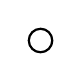
\begin{tikzpicture}[actor/.style={shape=circle,inner sep=3pt,draw, thick}]
	  \node (a) at (9,3) [actor] {};
	  \node [right] at (a.west) {\footnotesize};
	 \end{tikzpicture}
	 & \emph{Resource} \\	
		
	 \color{red}--- & \emph{Edge director} \\
	 \color{blue}--- & \emph{Edge actor} \\
	\end{tabular}	
\end{figure}
Si ottiene un nuovo multigrafo sparso direzionato di questo tipo:
\begin{figure}[H]
	\centering
	\begin{tikzpicture}
	[lineDecorate/.style={-,thick},%
	  film/.style={shape=diamond,inner sep=4pt,draw,thick, fill=blue!15}]
	
	%% nodes or vertices
	\foreach \nodename/\x/\y/\direction/\navigate in {
	  $Django Unchained$/0/4/left/west, $Inglourious Basterds$/4/4/right/east, $Titanic$/0/1/below/south}
	{
	  \node (\nodename) at (\x,\y) [film] {};
	  \node [\direction] at (\nodename.\navigate) {\small$\nodename$};
	}
	  \node ($actor Di Caprio actor$) at (0,2) {\color{red}\scriptsize{actor Di Caprio actor}};
	
	%% edges or lines
	\path
	\foreach \startnode/\endnode in {$Django Unchained$/$actor Di Caprio actor$,$actor Di Caprio actor$/$Titanic$}
	{
	  (\startnode) edge[lineDecorate,actor edge] node[] {} (\endnode)
	}
	
	\foreach \startnode/\endnode in {$Django Unchained$/$Inglourious Basterds$}
	{
	  (\startnode) edge[lineDecorate,bend left,actor edge] node[auto] {\scriptsize{actor Tarantino actor}} (\endnode)
	}
	
	\foreach \startnode/\endnode in {$Inglourious Basterds$/$Django Unchained$}
	{
	  (\startnode) edge[lineDecorate,bend left,director edge] node[auto] {\scriptsize{director Tarantino director}} (\endnode)
	};
	
	\end{tikzpicture}
\end{figure}

\begin{figure}[H]
	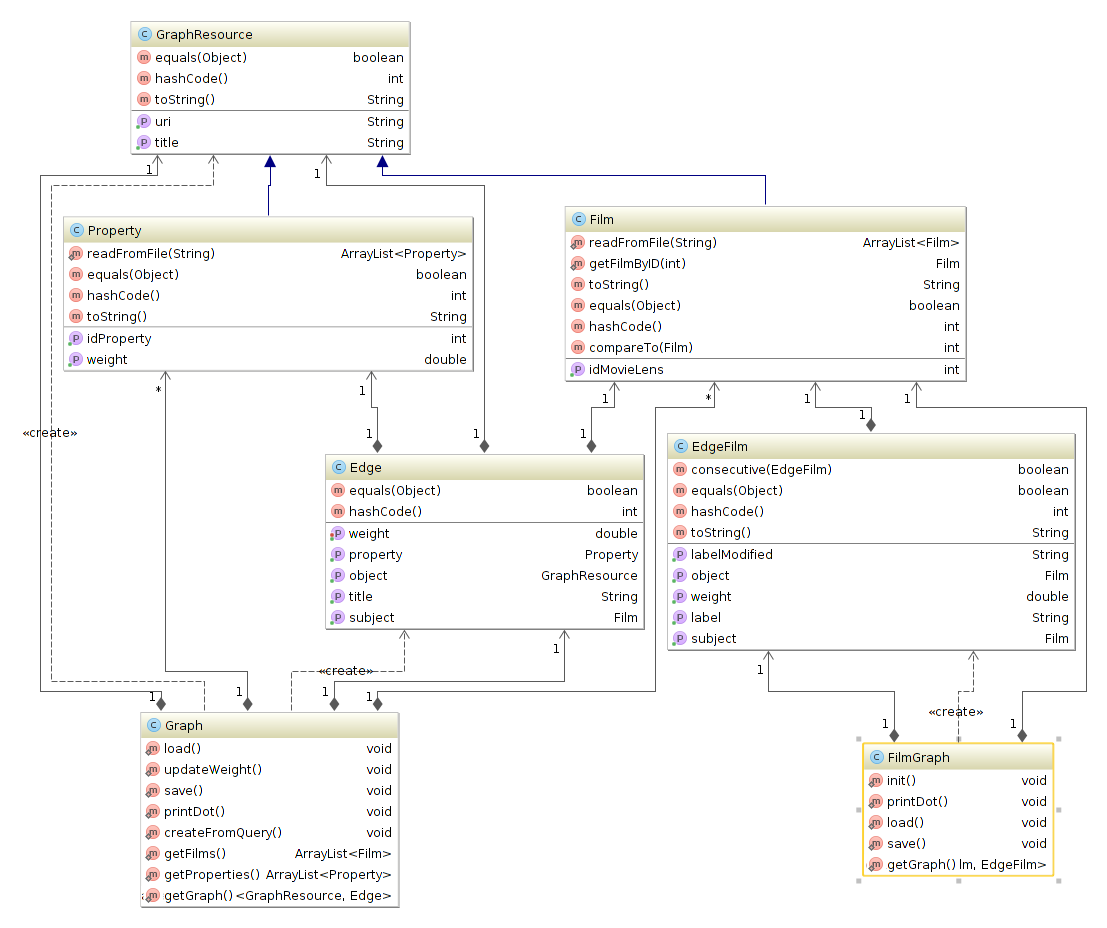
\includegraphics[width=\textwidth]{./images/Diagrams/graph.png}
	\caption{\emph{Class diagram: Package graph}}
\end{figure}

\subsection{Package distance}
\label{Package distance}
Il compito principale di questo package è quello di creare sia tutte le distanze di Passant (verranno definite nel dettaglio nei paragrafi \ref{PassantD} e \ref{PassantC}), sia le distanze da noi implementate (\ref{PassantDW} e \ref{PassantCW}). Per fare ciò, inizialmente verrà creato un hashmap tra la tipologia di distanza (PassantD, PassantC, PassantDW, ...) e l'oggetto \emph{distance} della relativa distanza; tale oggetto conterrà al suo interno un ulteriore hashmap tra la coppia di film e la relativa distanza che intercorre tra essi. In particolare, il metodo invocherà la classe astratta \emph{Distance} la quale, a sua volta, andrà ad implementare la relativa classe specifica.

\begin{figure}[H]
	\advance\leftskip-3cm
	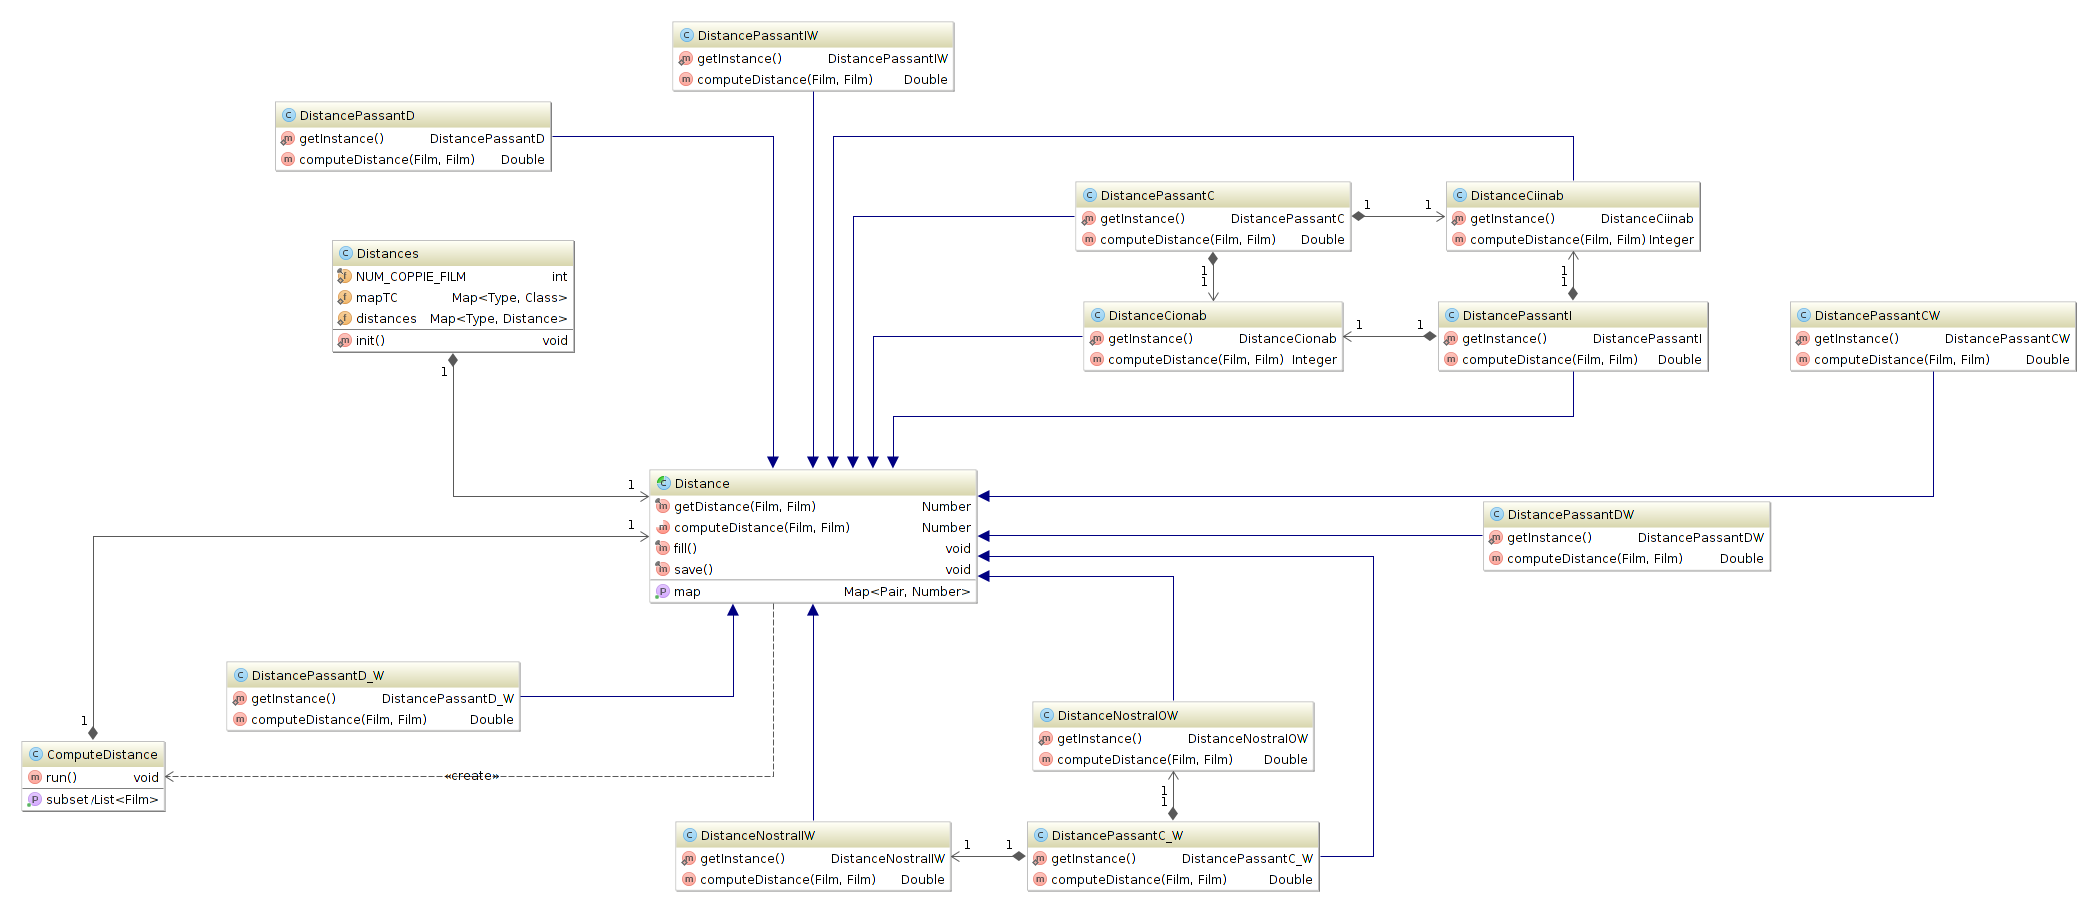
\includegraphics[width=1.45\textwidth]{./images/Diagrams/distance.png}
	\caption{\emph{Class diagram: Package distance}}
\end{figure}

\subsection{Package profile}
Tramite le classi presenti all'interno di questo package, sarà possibile implementare le due tipologie di profilo (pesato e non pesato)(verranno descritte in dettaglio nel paragrafo \ref{profili}). 

In particolare, con la classe \emph{ProfileNotWeighted} (estensione della classe \emph{Profile}), verranno create due collezioni di film nelle quali saranno presenti, in una i film votati positivamente, e nell'altra i film giudicati negativamente\footnote{I film presenti in entrambe le collezioni avranno peso uniforme.}; invece, con la classe \emph{ProfileWeighted}, anch'essa estensione della classe \emph{Profile}, si andrà a creare solo una collezione di film i quali avranno anche un attributo caratterizzante il peso del film in proporzione al voto dato, in particolare secondo la formula che verrà descritta nel paragrafo \ref{profili}. 
\begin{figure}[H]
	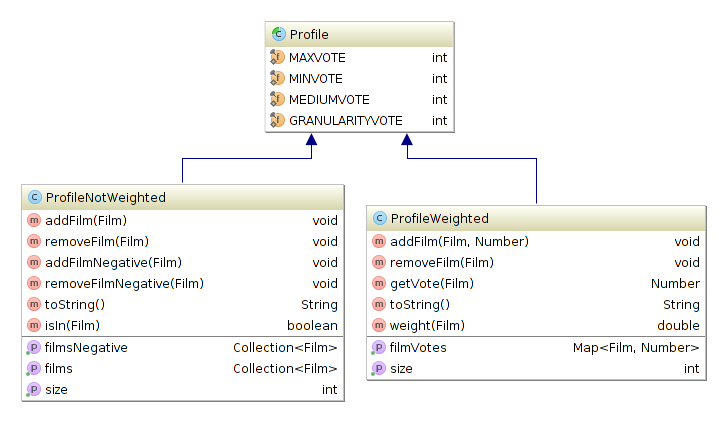
\includegraphics[width=\textwidth]{./images/Diagrams/profile.png}
	\caption{\emph{Class diagram: Package profile}}
\end{figure}

\subsection{Package recommendation}
Come dice il nome stesso, il compito di questo package consiste nella vera e propria fase di raccomandazione ad un utente partendo da una particolare configurazione. Per configurazione si intende definire innanzitutto ia tipologia di \emph{\textbf{distanza}} da utilizzare, poi quale tipo di profilo utente utilizzare (\emph{\textbf{pesato}} o \emph{\textbf{non pesato}}) e infine il numero \emph{\textbf{k}} di raccomandazioni da generare.

All'interno di questo package sono presenti essenzialmente due classi:
\begin{itemize}
\item \emph{Recommendation} 
\item \emph{Recommender}
\end{itemize} 
La prima ha lo scopo di definire la struttura dati che verrà restituita dalla raccomandazione; in particolar modo, restituirà la coppia Film-distanza, dove per \emph{Film} si intende la struttura dati contenente tutte le informazioni circa il film, quindi ID di movielens e URI di DBpedia a cui si riferisce; mentre per distanza si intende il valore numerico con precisione \emph{double} ottenuto dal calcolo delle distanze tra il film in questione e il film sorgente di riferimento.

La seconda classe invece, ha come obiettivo quello di effettuare la vera e propria raccomandazione, per fare ciò, si andrà a creare una struttura dati di tipo hashmap avente come primo parametro caratterizzante le diverse tipologie di distanze, mentre come secondo parametro un ulteriore hashmap aventi come parametro i diversi film e come secondo la lista di raccomandazioni partendo dal film utilizzato come parametro del secondo map e come distanza, il valore numerico ottenuto dal calcolo effettuato dal package distance definito precedentemente \ref{Package distance}. 

Graficamente la struttura dati può essere rappresentato in questo modo:

\begin{table}[H]
	\begin{tabular}{l | l | l | l }
	\emph{DISTANCE\_TYPE} & \emph{FILM\_SRC} & \emph{FILM\_DEST} & \emph{VAL\_DISTANCE} \\
	\toprule
		\multirow{6}{*}{PassantD} & \multirow{3}{*}{Film1} & Film2 & 0.9 \\
		&  & Film3 & 0.8 \\
		&  & Film4 & 0.7 \\ \cline{2-4}
		& \multirow{2}{*}{Film5} & Film6 & 0.95 \\ 
		& & Film7 & 0.8 \\
		& & Film8 & 0.7 \\ \bottomrule
		\multirow{6}{*}{PassantDW} & \multirow{3}{*}{Film1} & Film2 & 0.96 \\
		&  & Film4 & 0.91 \\ 
		&  & Film3 & 0.80 \\ \cline{2-4}
		& \multirow{2}{*}{Film5} & Film21 & 0.9 \\ 
		& & Film10 & 0.82 \\
		& & Film7 & 0.76 \\ \bottomrule
		... & ... & ... & ....
	\end{tabular}
\end{table}


\subsection{Package movielens\_exp}
Il package \emph{movielens\_exp} ha il compito di eseguire la vera e propria fase sperimentale del progetto; innanzitutto viene eseguita la fase di splitting delle votazioni date da ogni utente ai vari film visionati allo scopo di creare i set di training e di test. Successivamente si passa alla creazione dei profili(\emph{pesato} e \emph{non pesato}) partendo dalle votazioni presenti all'interno del training set di ogni utente; infine nella parte finale della sperimentazione vengono calcolate le diverse tipologie di metriche descritte in \ref{metriche}.

